\section{Дослідження розроблених алгоритмів}

\subsection{Дослідження моделі похибок БІНС}

Перевіримо модель та впливи різних складових похибок, на модель БІНС, зобразимо їх в
залежності від часу. Моделювання проведемо над стаціонарно закріпленою БІНС.
Для початку перевіримо випадок коли координатний тригранник має невеликий нахил,
помилку $\Delta \alpha_{E}$. Це призведе до того, що на горизонтальний акселерометр
подіє прискорення $-g \alpha_{E}$. Виміряне прискорення спричинить, до того, що після
двох інтеграторів, буде здаватись, що система має швидкість і відповідно рухається.
Це спричинить момент на гіроскопах в напрямку зменшення зміщення помилки
координатного тригранника, але коли акселерометр стає зрівноваженим система 
матиме значну швидкість, що продовжить коливання. Це нагадує маятник, коли відхиляють
підвіс і дають йому коливатись

\begin{figure}[here]
\centering
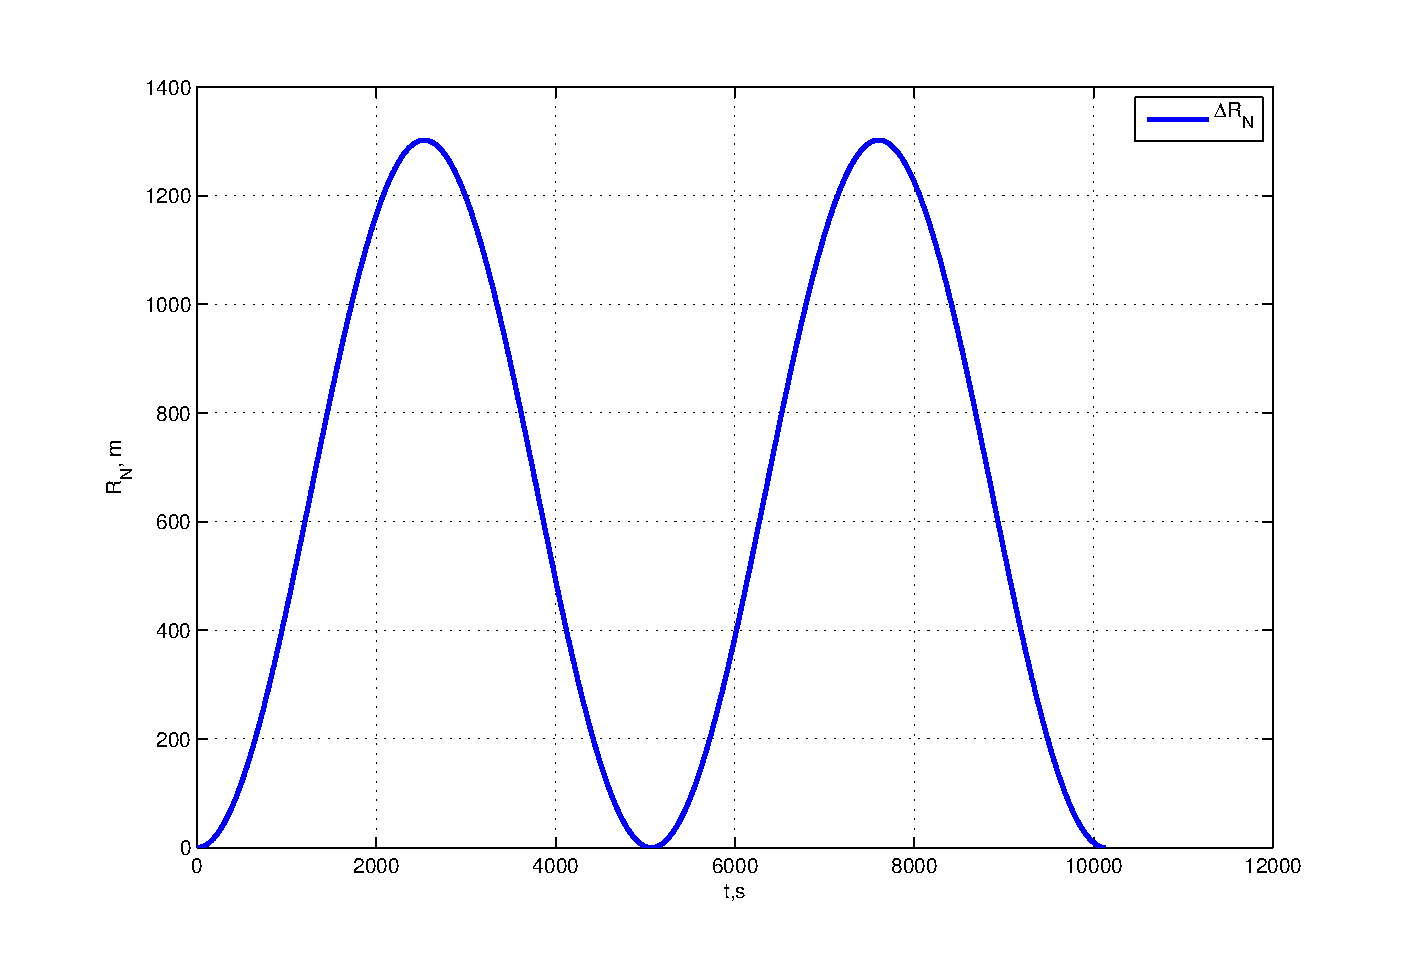
\includegraphics[scale=0.4]{ins_stat_tilt}
\caption{Еволюція похибки за умови, похибки координатного тригранника $10^{-3} rad$}
\label{fig:ins_stat_tilt}
\end{figure}

На рис. \ref{fig:ins_stat_tilt} зображено результат моделювання руху похибки ІНС
яка зумовлена початковим зміщенням координатного тригранника на $10^{-3} rad$.
Можна зазначити, що помилка коливається з частотою Шулера, з періодом 84.4 хвилини.
Найбільша помилка приблизно 1300 метрів і досягається приблизно за 42.2 хвилини роботи системи.

Розглянемо еволюцію похибок при наявності дрейфу гіроскопа. Ефект дрейфу гіроскопа позначається на нахилі координатного тригранника, в результаті виникає помилка прискорення. Швидкість і координата коливаються з частотою Шулера. Але цього разу швидкість
коливається не навколо нуля, отже помилка координати утворюється як сума лінійної наростаючої та гармонічної функції.

 Яскраво виражені коливання Шулера та лінійно наростаюча функція на рис.\ref{fig:ins_stat_gyro} як загальна помилка для стаціонарно закріпленої ІНС з дрейфом вертикального гіроскопа на $0.01^{o}/h$,. Після 1 години роботи похибка по координаті приблизно 1300 метрів. Якщо гіроскоп менш точний то його дрейф спричиняє похибку 1600 метрів за 10 хвилин. Зрозуміло, що на не дорогих ДПІ похибка зростає до 1500 метрів за 1 хвилину.
\begin{figure}[here]
\centering
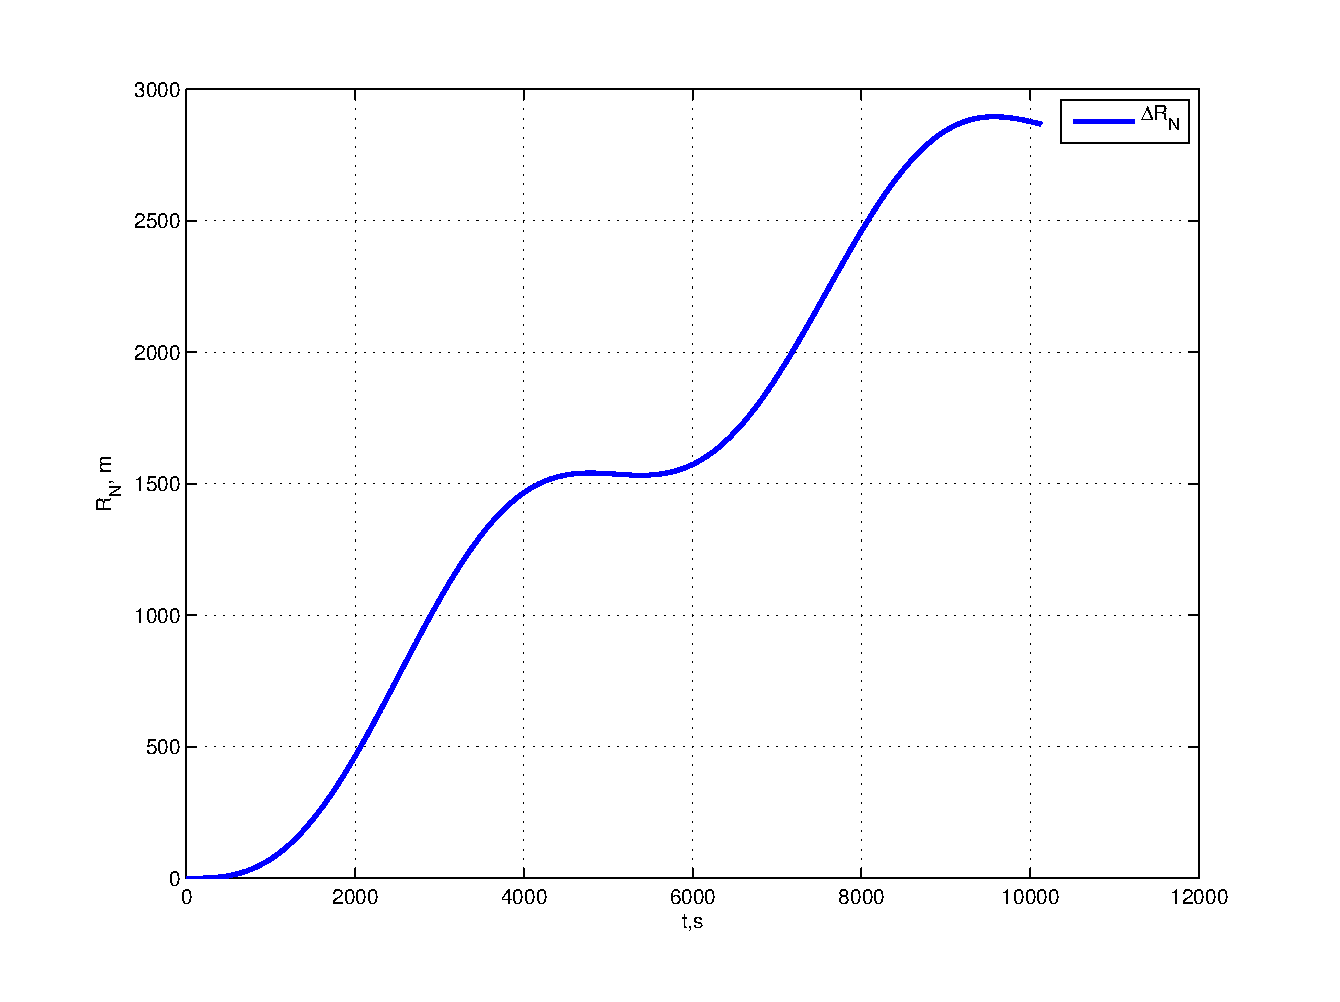
\includegraphics[scale=0.4]{ins_stat_gyro}
\caption{Еволюція похибки за умови, дрейфу гіроскопа $0.01 deg/h$}
\label{fig:ins_stat_gyro}
\end{figure}

При наявності помилки по швидкості $\Delta V_{E} =1$ м/с позиційна похибка буде обмеженою і коливатиметься з частотою Шулера рис.\ref{fig:ins_stat_velo}.
\begin{figure}[here]
\centering
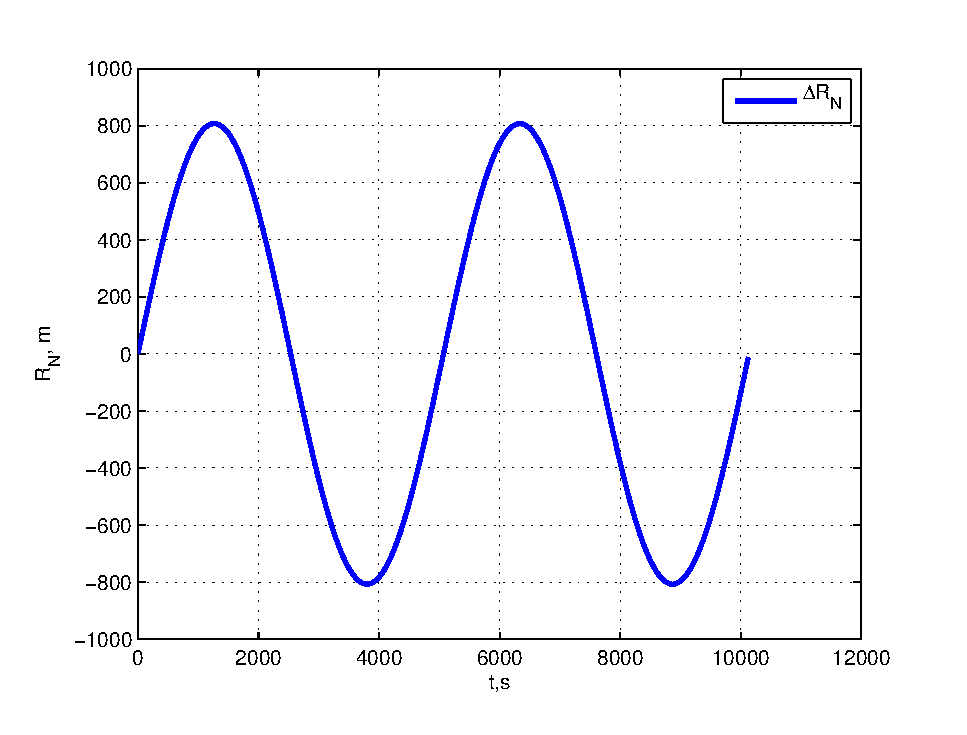
\includegraphics[scale=0.5]{ins_stat_velo}
\caption{Еволюція похибки при початковій похибці по швидкості 1 м/с}
\label{fig:ins_stat_velo}
\end{figure}

Далі порівняємо ефект впливу помилок різного типу в стаціонарно закріпленій ІНС. На рис. \ref{fig:ins_stat_sum}.
На малюнку зображено вплив кожного виду помилки: помилку початкової виставки як помилку нахилу координатного тригранника та помилки ДПІ як дрейфи акселерометра та гіроскопа. Також результуючу помилку по координаті, як суму перерахованих вище.
\begin{figure}[H]
\centering
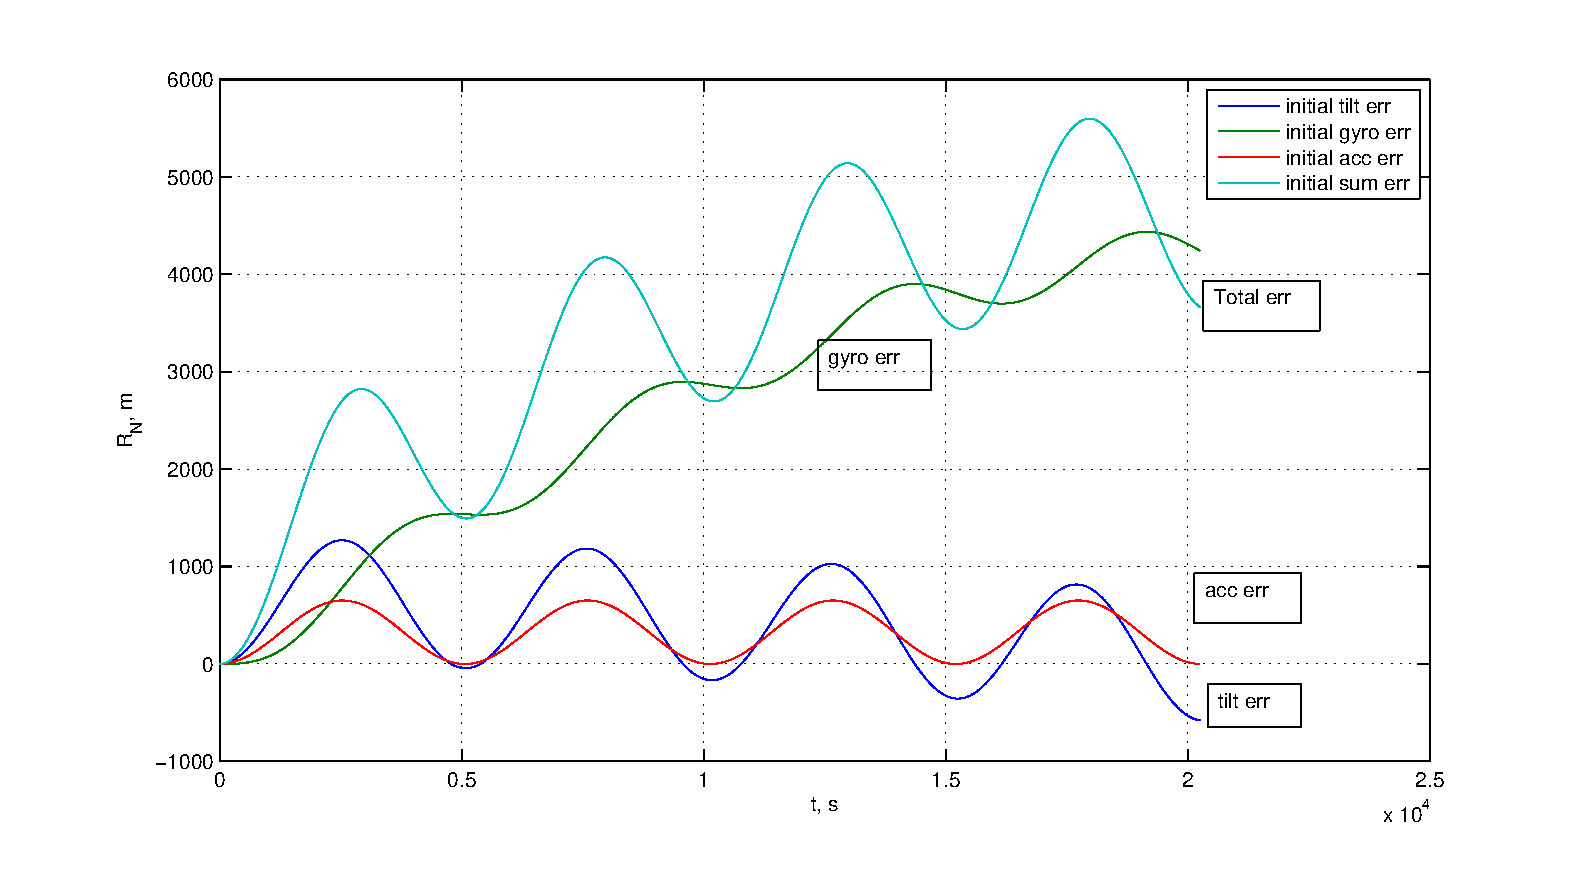
\includegraphics[scale=0.67]{ins_stat_sum}
\caption{Еволюція сумарної похибки по координаті за умови,
дрейфу гіроскопа   $0.01 deg/h$,похибки координатного тригранника $10^{-3} rad$, та зміщенням акселерометра $10^{-4} rad$ }\label{fig:ins_stat_sum}
\end{figure}

Можна зауважити, що за виключенням початкової виставки, сумарна похибка по координаті переважно визначається дрейфом гіроскопа. Дрейф інтегрується один раз, коли розраховується кут для перетворення прискорення, який потім інтегрується вдруге для отримання позиційної похибки.

\subsection{Рівняння траєкторії ЛА}

Еталонні параметри руху ЛА у функції часу задавалися аналітично, що дозволило уникнути методичних похибок у процесі моделювання.

Географічні координати описуються наступними рівняннями:
\begin{equation}
\label{emu_path_pos} 
\begin{array}{l} 
{\varphi (t)=\varphi_{0}+K_{\varphi } t+\Delta_{\varphi } \sin (\omega_{\varphi } t+\delta_{\varphi } );} \\ 
{\lambda (t)=\lambda_{0}+K_{\lambda } t+\Delta_{\lambda } \sin (\omega_{\lambda } t+\delta_{_{\lambda } } );} \\ 
{h(t)=h_{0} -\Delta h \cos (\omega_{h} t+\delta_{h} );} \\ 
{\omega _{\varphi } =2\pi /T_{\varphi } ;} \\ {\omega _{\lambda } =2\pi /T_{\lambda } ;} \\ 
{\omega _{h} =2\pi /T_{h} ;} 
\end{array}
\end{equation}

Складові швидкості руху відносно Землі:
\begin{equation}
\label{emu_path_vel} 
\begin{array}{l}
{V_{E} (t)=\dot{\lambda }(t)\left[R_{1} (\varphi )+h(t)\right]\cos \varphi (t);} \\ 
{V_{N} (t)=\dot{\varphi }(t)[R_{2} (\varphi )+h(t)];} \\ 
{V_{h} (t)=\dot{h}(t);} \\ {R_{1} (\varphi )=\frac{a}{\sqrt{1-e^{2} \sin ^{2} \varphi } } ;} \\ 
{R_{2} (\varphi )=R_{1} (\varphi )\frac{1-e^{2} }{1-e^{2} \sin ^{2} \varphi } ;} 
\end{array} 
\end{equation}

Де a та $e^2$ велика полувісь та квадрат першого ексцентриситету земного еліпсоїда: 
\begin{itemize}
 \item для: СК-42: $a=6378245$м,  $e^2=6,69342749\cdotp 10^{-3}$
 \item для: ПЗ-90: $a=6378136$м,  $e^2=6,69436619\cdotp 10^{-3}$
 \item для: WGS-84: $a=6378137$м, $e^2=6,6943799901413\cdotp 10^{-3}$
\end{itemize}

Складові уявного прискорення:
\begin{equation}
\label{emu_path_acc} 
\begin{array}{l} 
{a_{E}(t)=\dot{V}_{E} (t)-q(t)\sin \varphi (t)V_{N} (t)+q(t)\cos (t)V_{h} (t);} \\ 
{a_{N}(t)=\dot{V}_{N} (t)+q(t)\sin \varphi (t)V_{E} (t)+\dot{\varphi }(t)V_{h} (t);} \\ 
{a_{h}(t)=\dot{V}_{h} (t)-q(t)\cos \varphi (t)V_{E} (t)-\dot{\varphi }(t)V_{N} (t)+g(h,\varphi);} \\ 
{q(t)=\dot{\lambda }(t)+2\omega_{3} ;} \\ 
{g(h,\varphi)=g_{e} [1-2\frac{h(t)}{a} +\frac{3}{4} e^{2} \sin ^{2} \varphi (t)];} 
\end{array}
\end{equation}
\begin{ESKDexplanation}
\item де $g_{e} =\frac{\mu }{a^{2} }$, $\mu =398600.44\cdot 10^{9} $
\item $\omega_{\text{З}} $ -- кутова швидкість обертання Землі.
\end{ESKDexplanation}
\begin{equation}
\label{emu_path_dv} 
\begin{array}{l} 
{\dot{V}_{E} (t)=\ddot{\lambda}(t)[R_{1}(\varphi)+h(t)]\cos (t)+}\\
{+\dot{\lambda}(t)[\dot{R}_{1}(\varphi )+V_{h} (t)]\cos(t)-}\\
{-\dot{\lambda}(t)[R_{1} (\varphi )+h(t)]\sin \varphi \cdotp \dot{\varphi}(t);} \\ 
{\dot{V}_{N}(t)=\ddot{\varphi}(t)[R_{2}(\varphi )+h(t)]+\dot{\varphi}(t)[\dot{R}_{2} (\varphi )+V_{h}(t)];} \\ 
{\dot{V}_{h}(t)=\ddot{h}(t);} \\ 
{\dot{R}_{1} (t)=\frac{ae^{2} \sin \varphi (t)\cdot \cos y(t)\cdot \dot{\varphi }(t)}{(1-e^{2} \sin ^{2} \varphi)^{3/2}};}\\ 
{\dot{R}_{2} =\dot{R}_{1} (t)\frac{1-e^{2} }{1-e^{2} \sin ^{2} \varphi} +R_{1} (\varphi)\frac{(1-e^{2} )2e^{2} \sin \varphi \cdot \cos \varphi \cdot \dot{y}(t)}{(1-e^{2} \sin ^{2} \varphi )^{2}} ;} 

\end{array}
\end{equation} 

Кути тангажа, курса та крена (вважається, що поздовжня ось об’єкта спів-падає з вектором відносної швидкості, а кут крена пропорційний боковому прискоренню) визначаються з наступних співвідношень:

\begin{equation}\label{emu_path_pyr} 
\begin{array}{l} 
{\vartheta(t)=arctg[V_{h} (t)/V_{r} (t)];} \\ 
{\psi (t)=arctg[V_{E}(t)/V_{N} (t)];} \\ 
{\gamma (t)=K_{\gamma }\frac{V_{N}(t)\dot{V}_{E}(t)-V_{E}(t)\dot{V}_{N}(t)}{V_{r}(t)\cos v(t)},}
 \end{array}\end{equation} 
\begin{ESKDexplanation}
\item де $V_{r}(t)=\sqrt{V_{N}^{2} (t)+V_{E}^{2} (t)}$
\item $K_{\gamma}\approx 0.02$  рад/(м/$c^2$).
\end{ESKDexplanation}

Супутникова навігаційна система надає вимірювання швидкостей і координат, що є не достатнім для оцінки параметрів, які безпосередньо не спостерігаються (дрейфи гіроскопів і зміщення акселерометрів), але при виконанні певних маневрів, рівень спостережності збільшується. Наприклад, в роботі \cite{bib:observ} проводиться аналіз спостережності стану змінної в часі системи в залежності від маневрів ЛА, з чого можна зробити висновок, що обертання ЛА навколо трьох осей має найбільший рівень спостережності. Отже дані при спостереженні дрейфів ДПІ може бути використано для їх польотного калібрування. 

Беручі до уваги вище зазначене, пропонується наступна тестова траєкторія рисунку \ref{fig:path_3d}:

\begin{figure}[H]
\centering
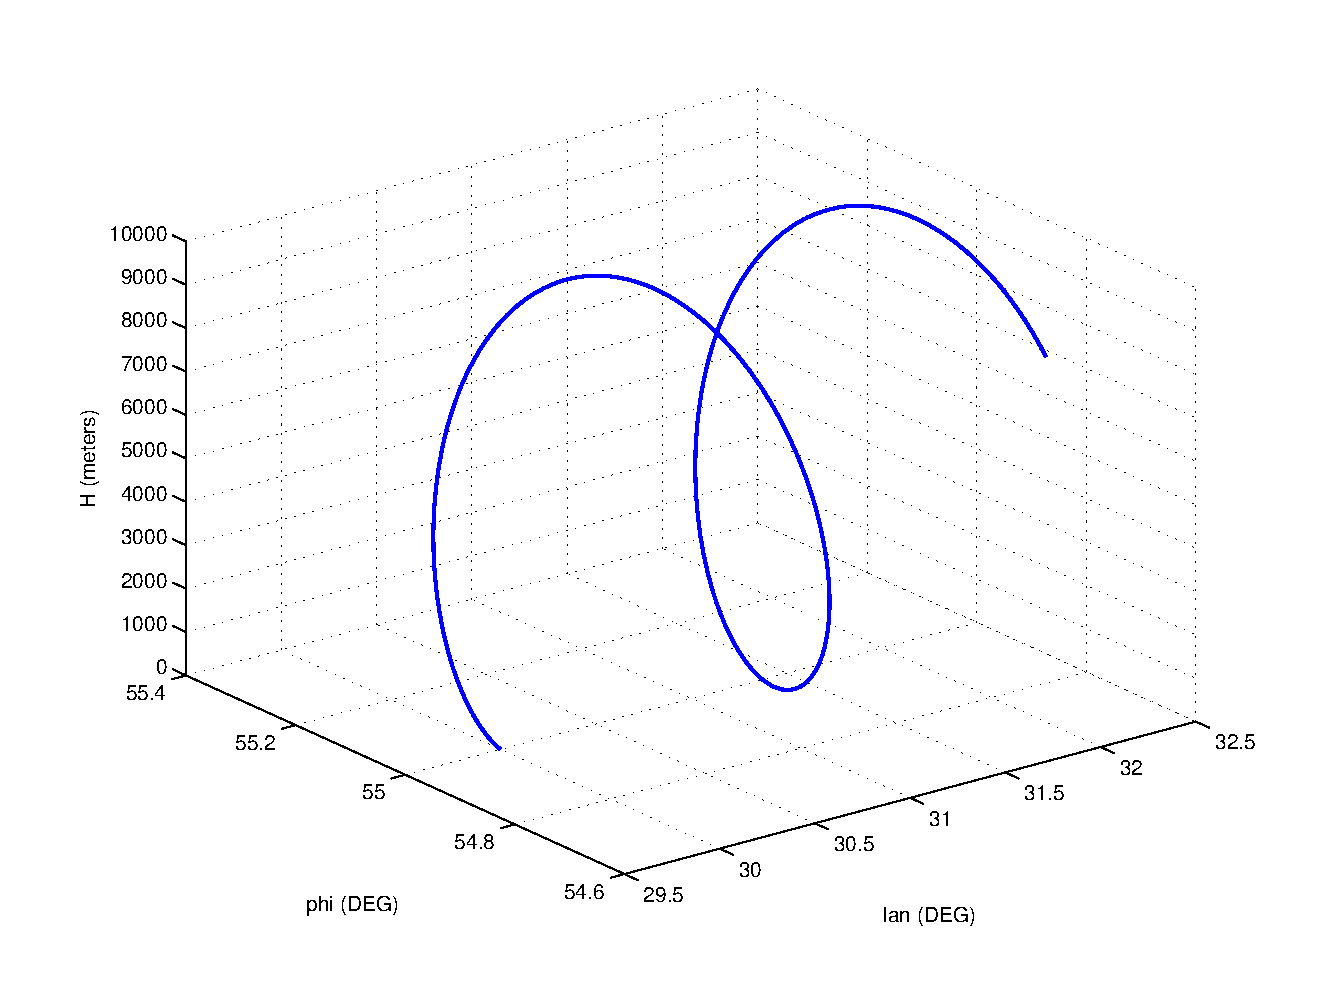
\includegraphics[scale=0.6]{path_3d}
\caption{Траєкторія руху ЛА}
\label{fig:path_3d}
\end{figure}
Кути курсу, крену тажгажа мають наступну залежність від часу рис\ref{fig:path_PYR}:
\begin{figure}[H]
\centering
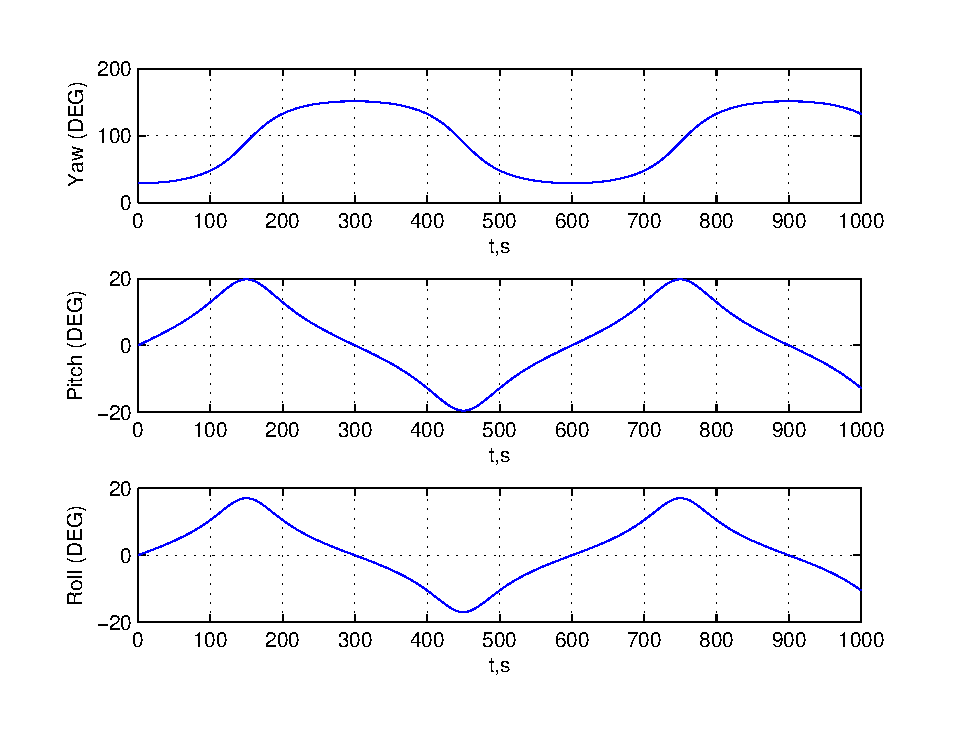
\includegraphics[scale=0.8]{path_PYR}
\caption{Залежність курса, тангажа та крена від часу}
\label{fig:path_PYR}
\end{figure}

\begin{itemize}
\item $\varphi_{0}=55^{o}$ $\lambda_{0}=30^{o}$ -- координати передмістя Києва;
\item $T_{\varphi } = 600$; $T_{\lambda } =  600$; $T_{h} =  600$;
\item $h0 = 5000$; $K_{\varphi } = 0$; $K_{\lambda } = 0.00004$;
\item $\Delta \varphi =0.004$; $\Delta \lambda = 0$; $\Delta h = h0$;
\item $\delta \varphi = 0$; $\delta \lambda =0$; $\delta h =0$ ;
\end{itemize}

\subsection{Моделювання алгоритмів калманівської фільтрації}

Нижче представлені результати імітаційного моделювання алгоритмів калманівської фільтрації при побудові інваріантного алгоритму комплексної обробки інформації на прикладі польоту ЛА за заданою траєкторією. На рис \ref{fig:ErrEstCovR}...\ref{fig:ErrEstCovAcc} представлено еволюції похибок оцінювання: координат та висоти польоту (рис.\ref{fig:ErrEstCovR}), складових швидкості (рис.\ref{fig:ErrEstCovV}), параметрів кутової орієнтації (рис. \ref{fig:ErrEstCovAlph}), вихідних сигналів гіроскопів (рис. \ref{fig:ErrEstCovGyro}), акселерометрів (рис. \ref{fig:ErrEstCovAcc}).

\begin{figure}[H]
\centering
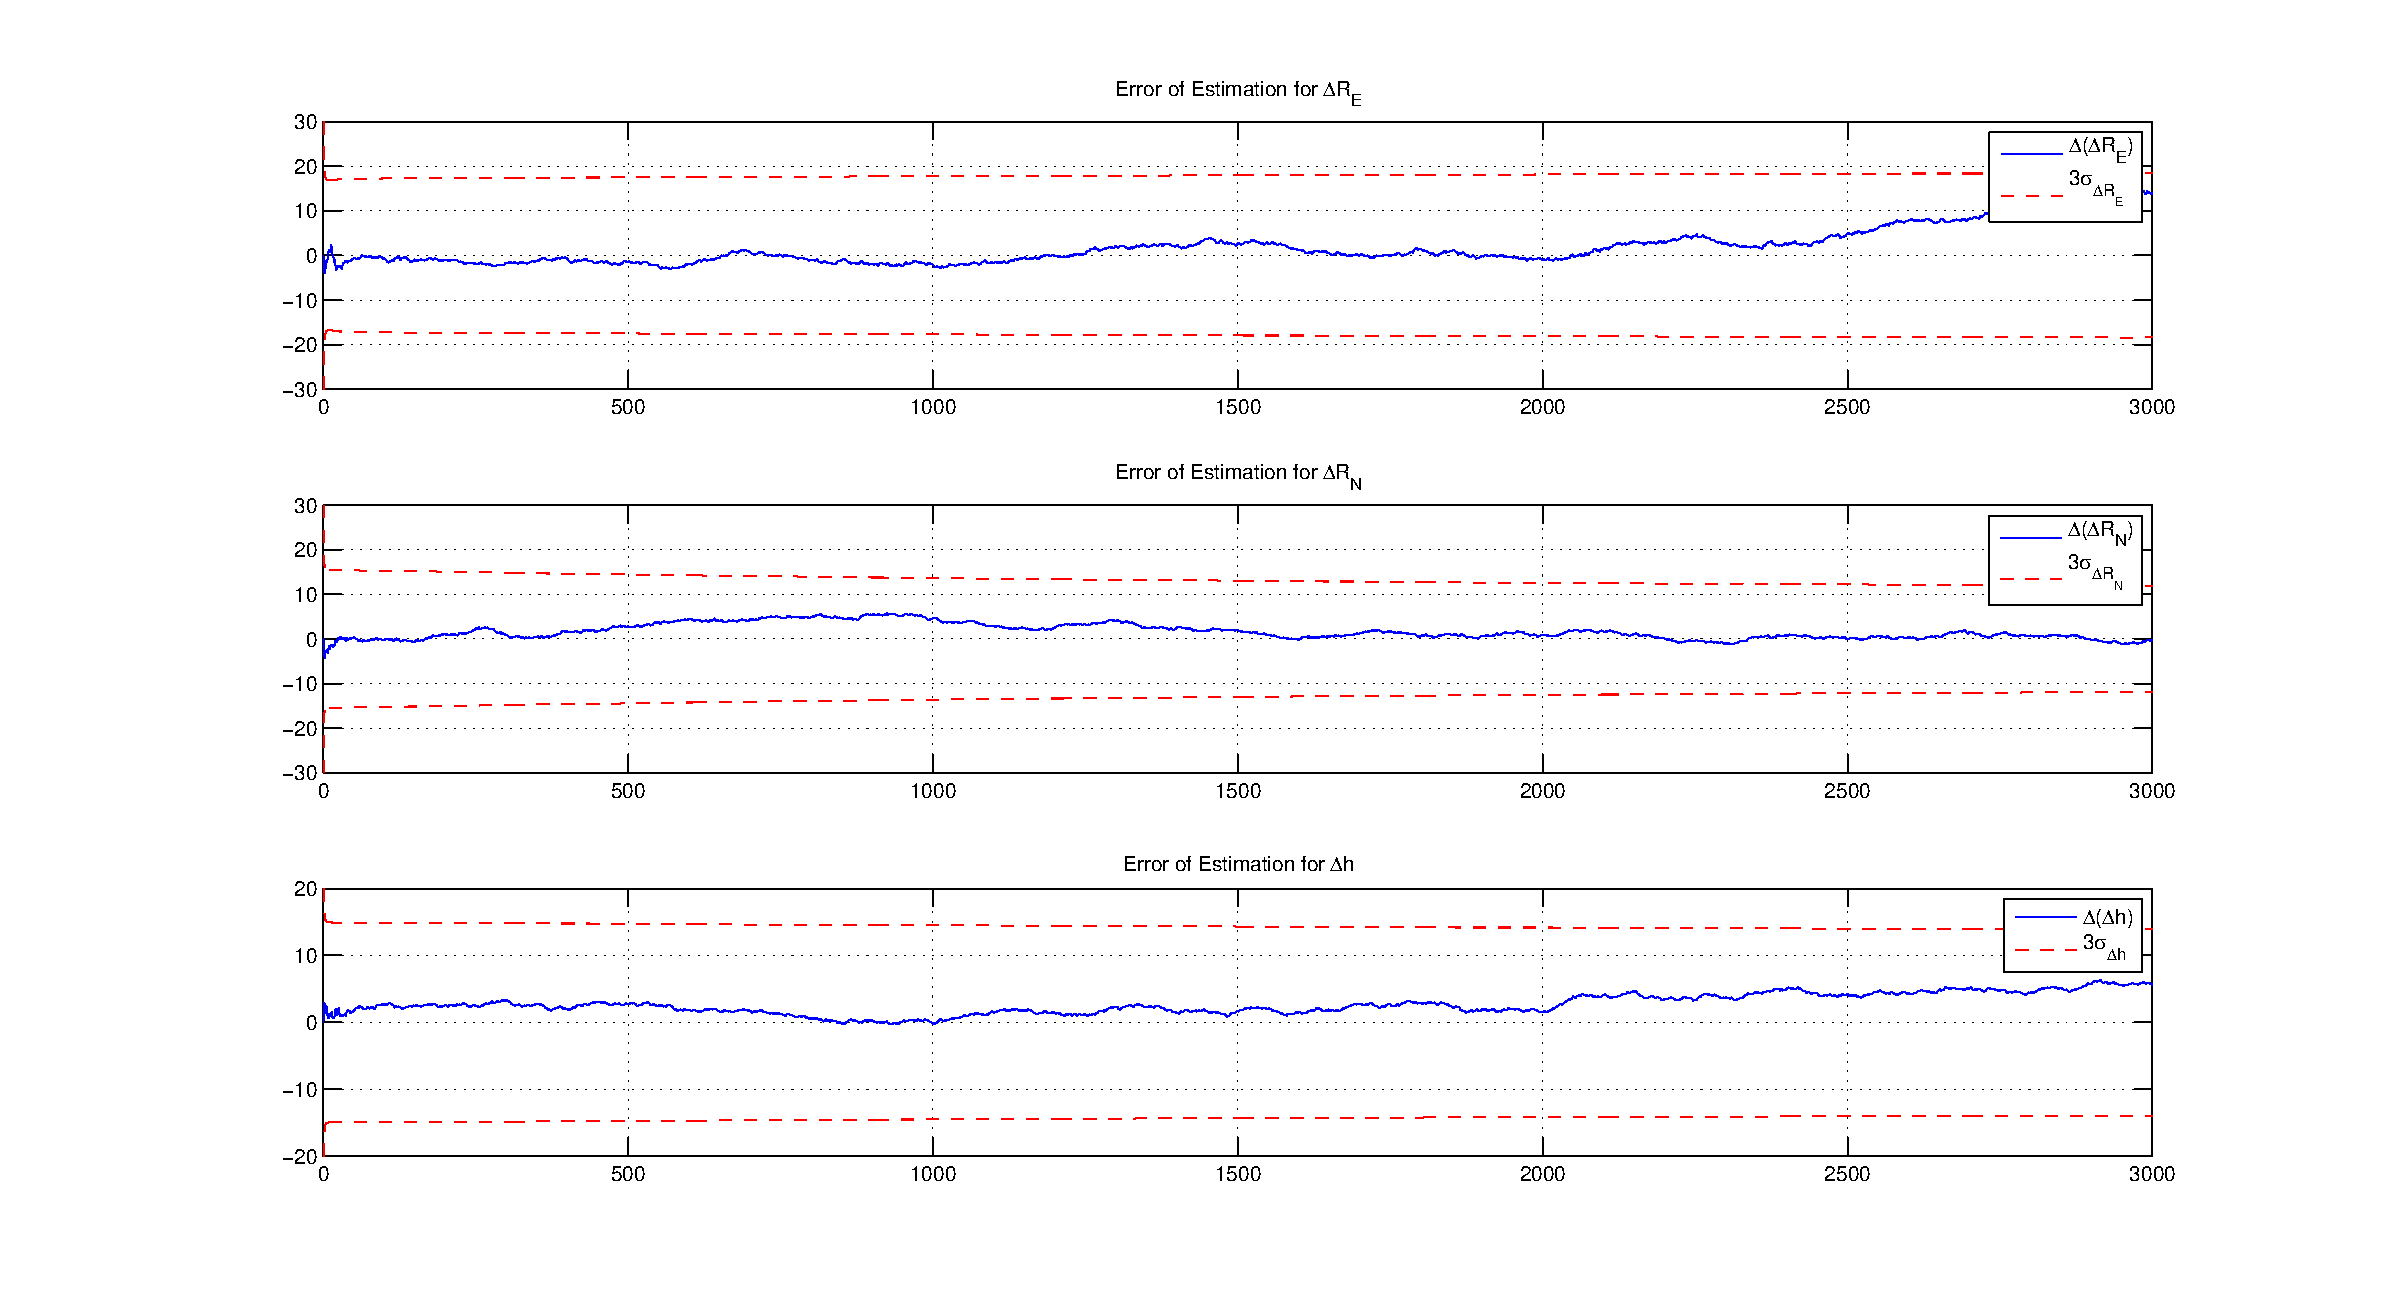
\includegraphics[scale=0.45]{ErrEstCovR}
\caption{Еволюції похибок координат}
\label{fig:ErrEstCovR}
\end{figure}
\begin{figure}[H]
\centering
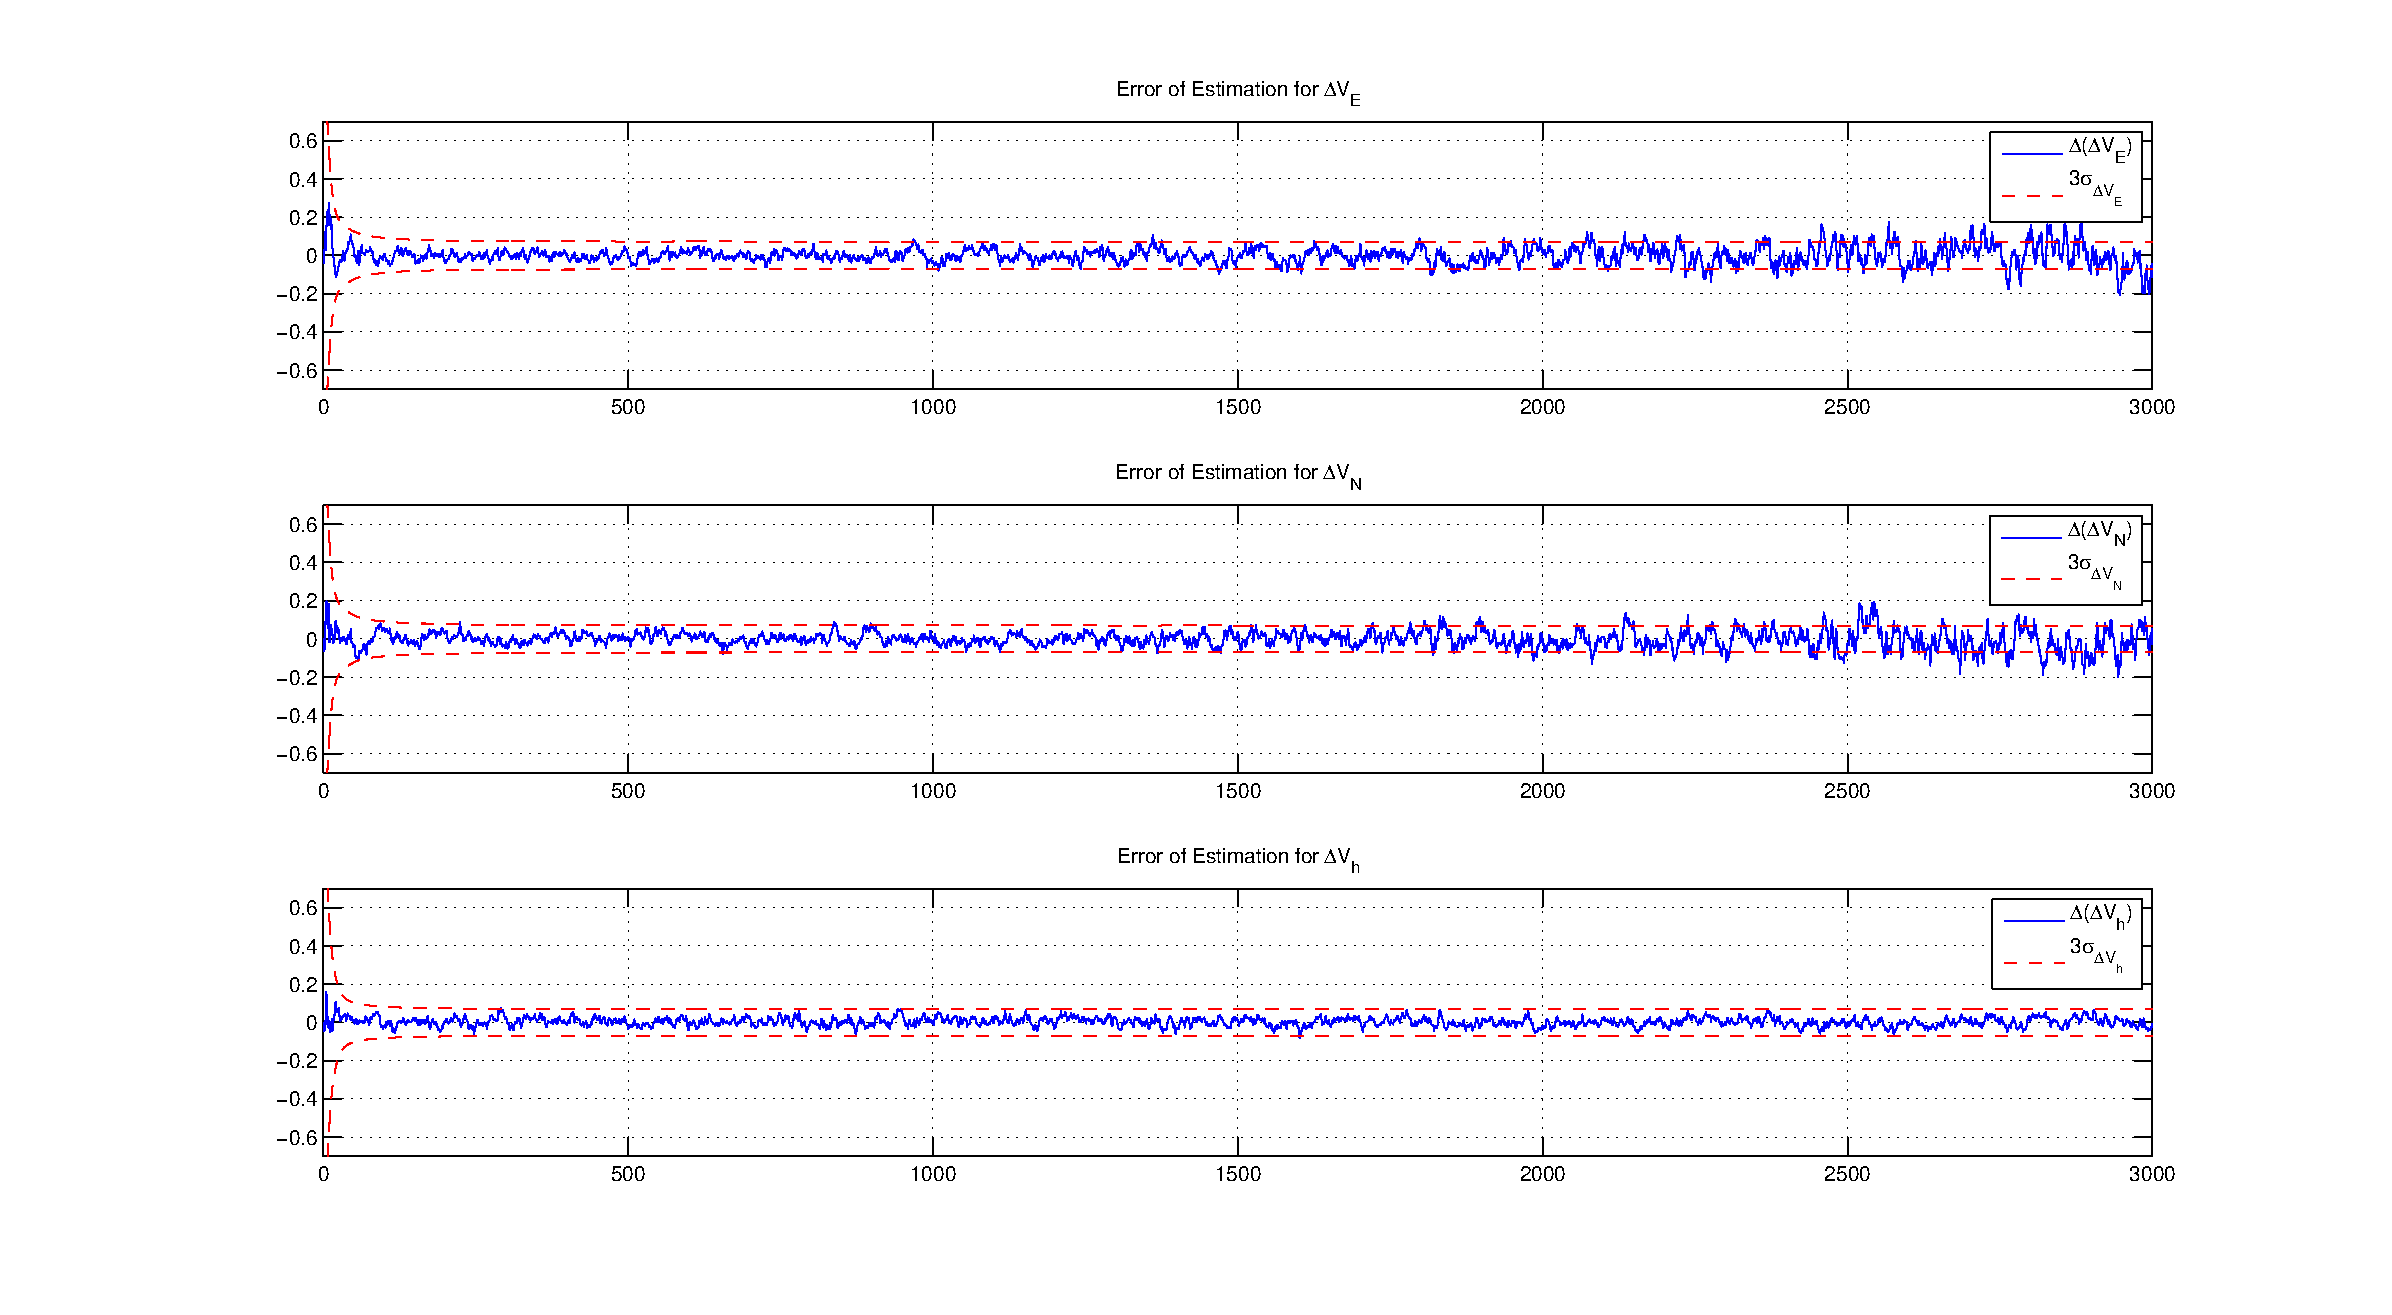
\includegraphics[scale=0.45]{ErrEstCovV}
\caption{Еволюції похибок швидкостей}
\label{fig:ErrEstCovV}
\end{figure}

\begin{figure}[H]
\centering
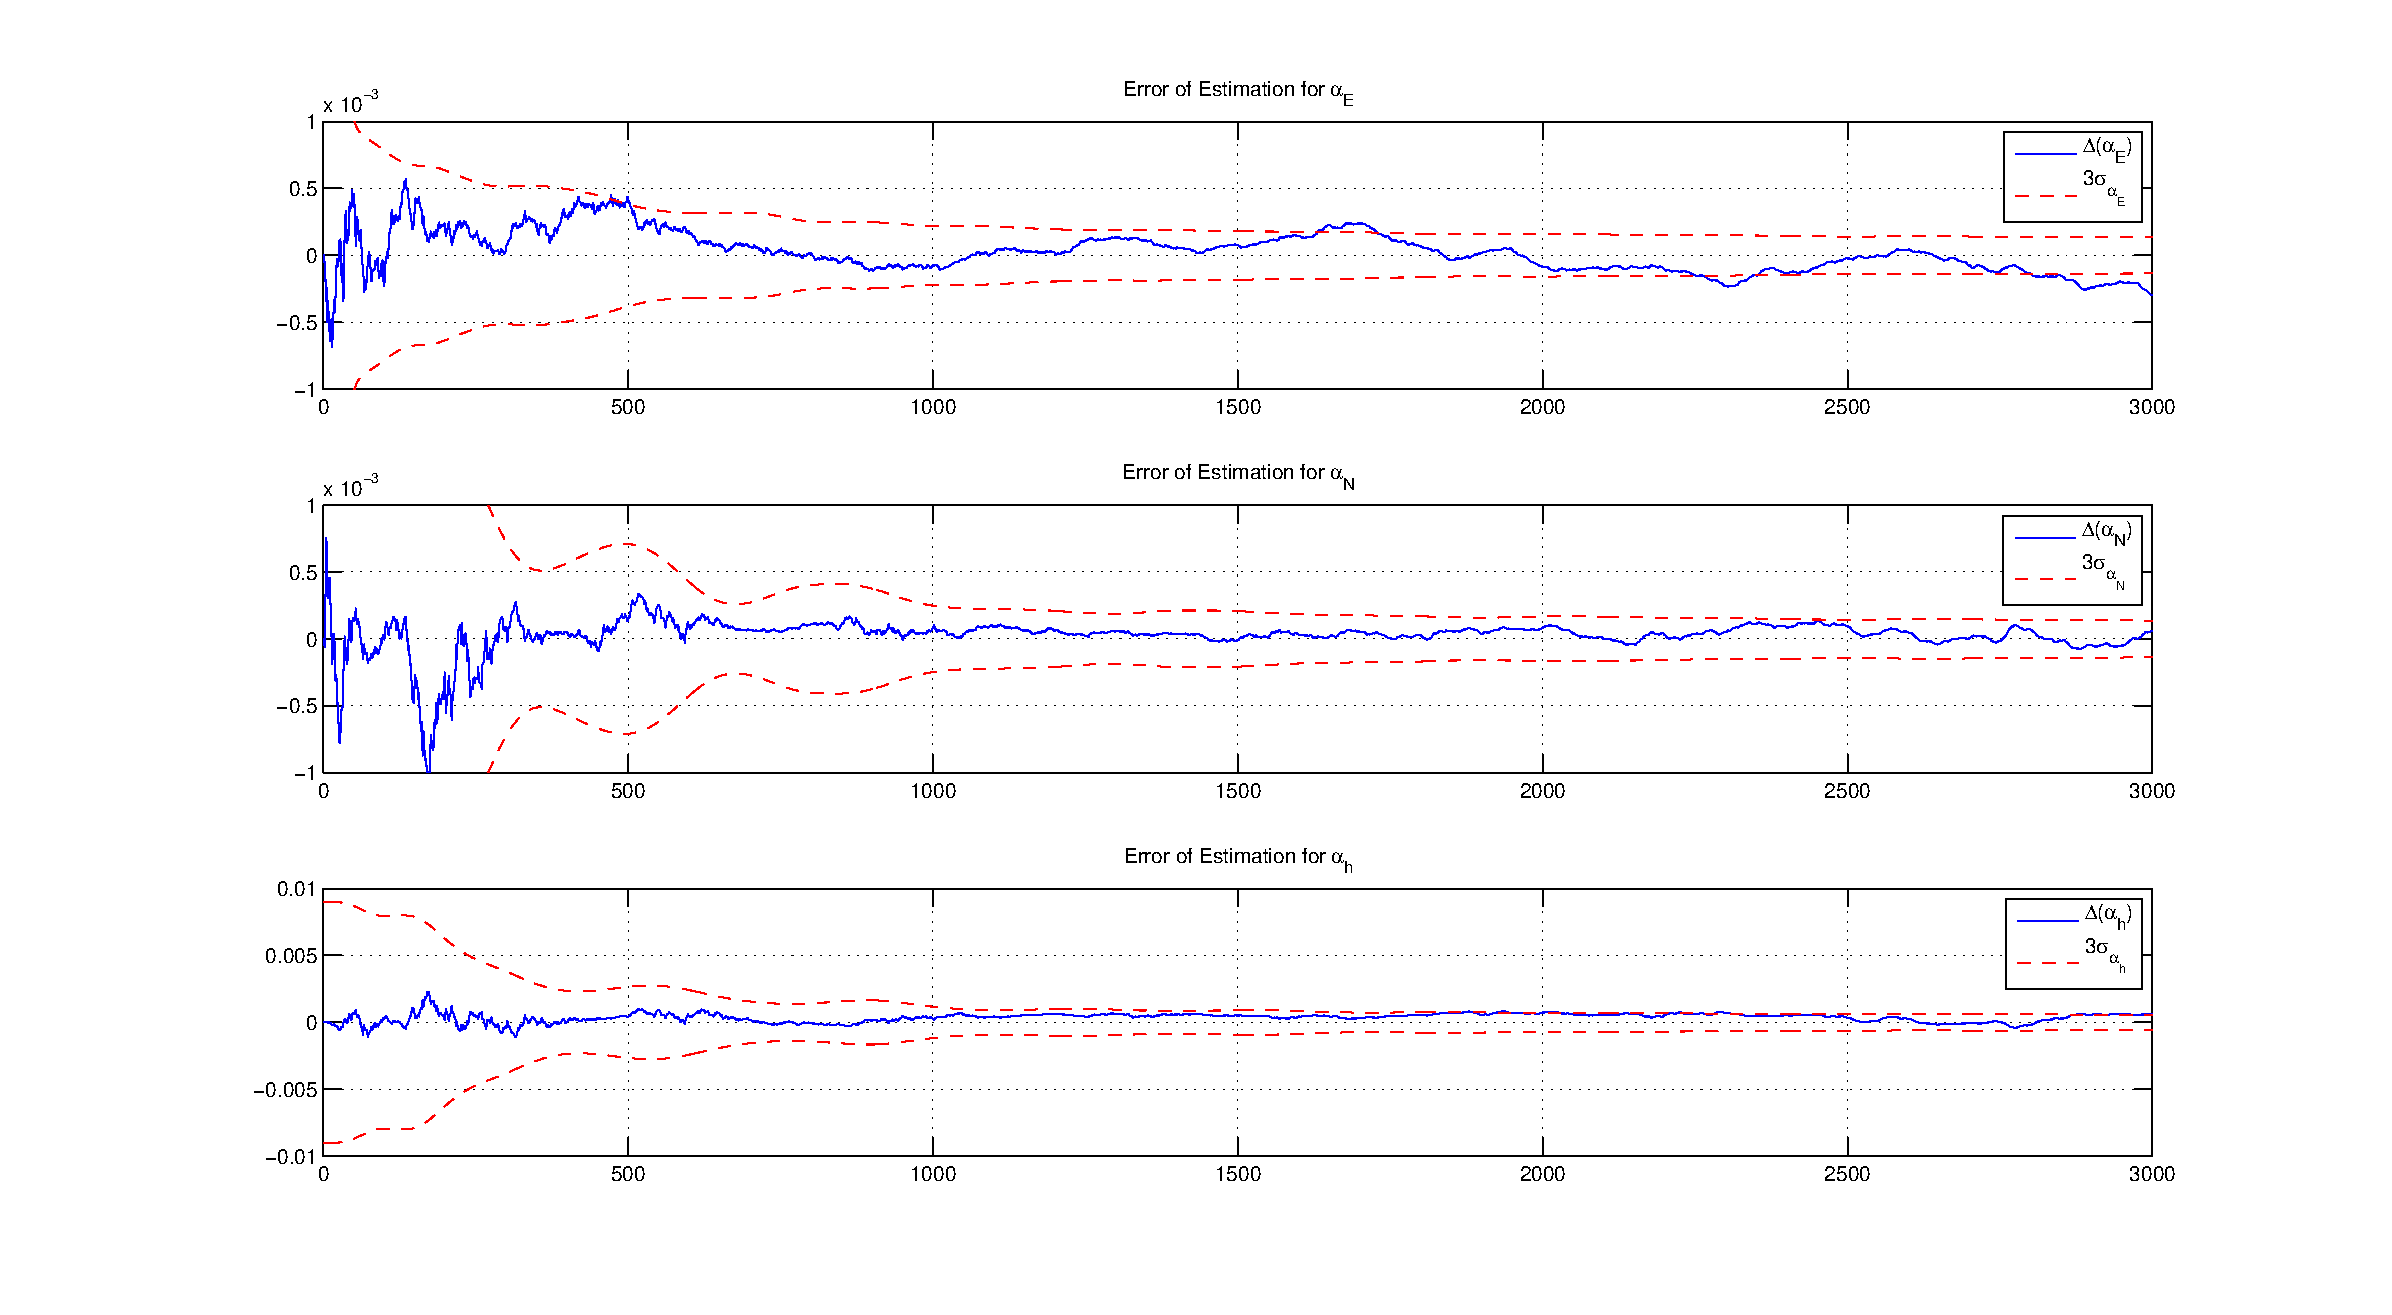
\includegraphics[scale=0.45]{ErrEstCovAlph}
\caption{Еволюції похибок параметрів кутової орієнтації}
\label{fig:ErrEstCovAlph}
\end{figure}

\begin{figure}[H]
\centering
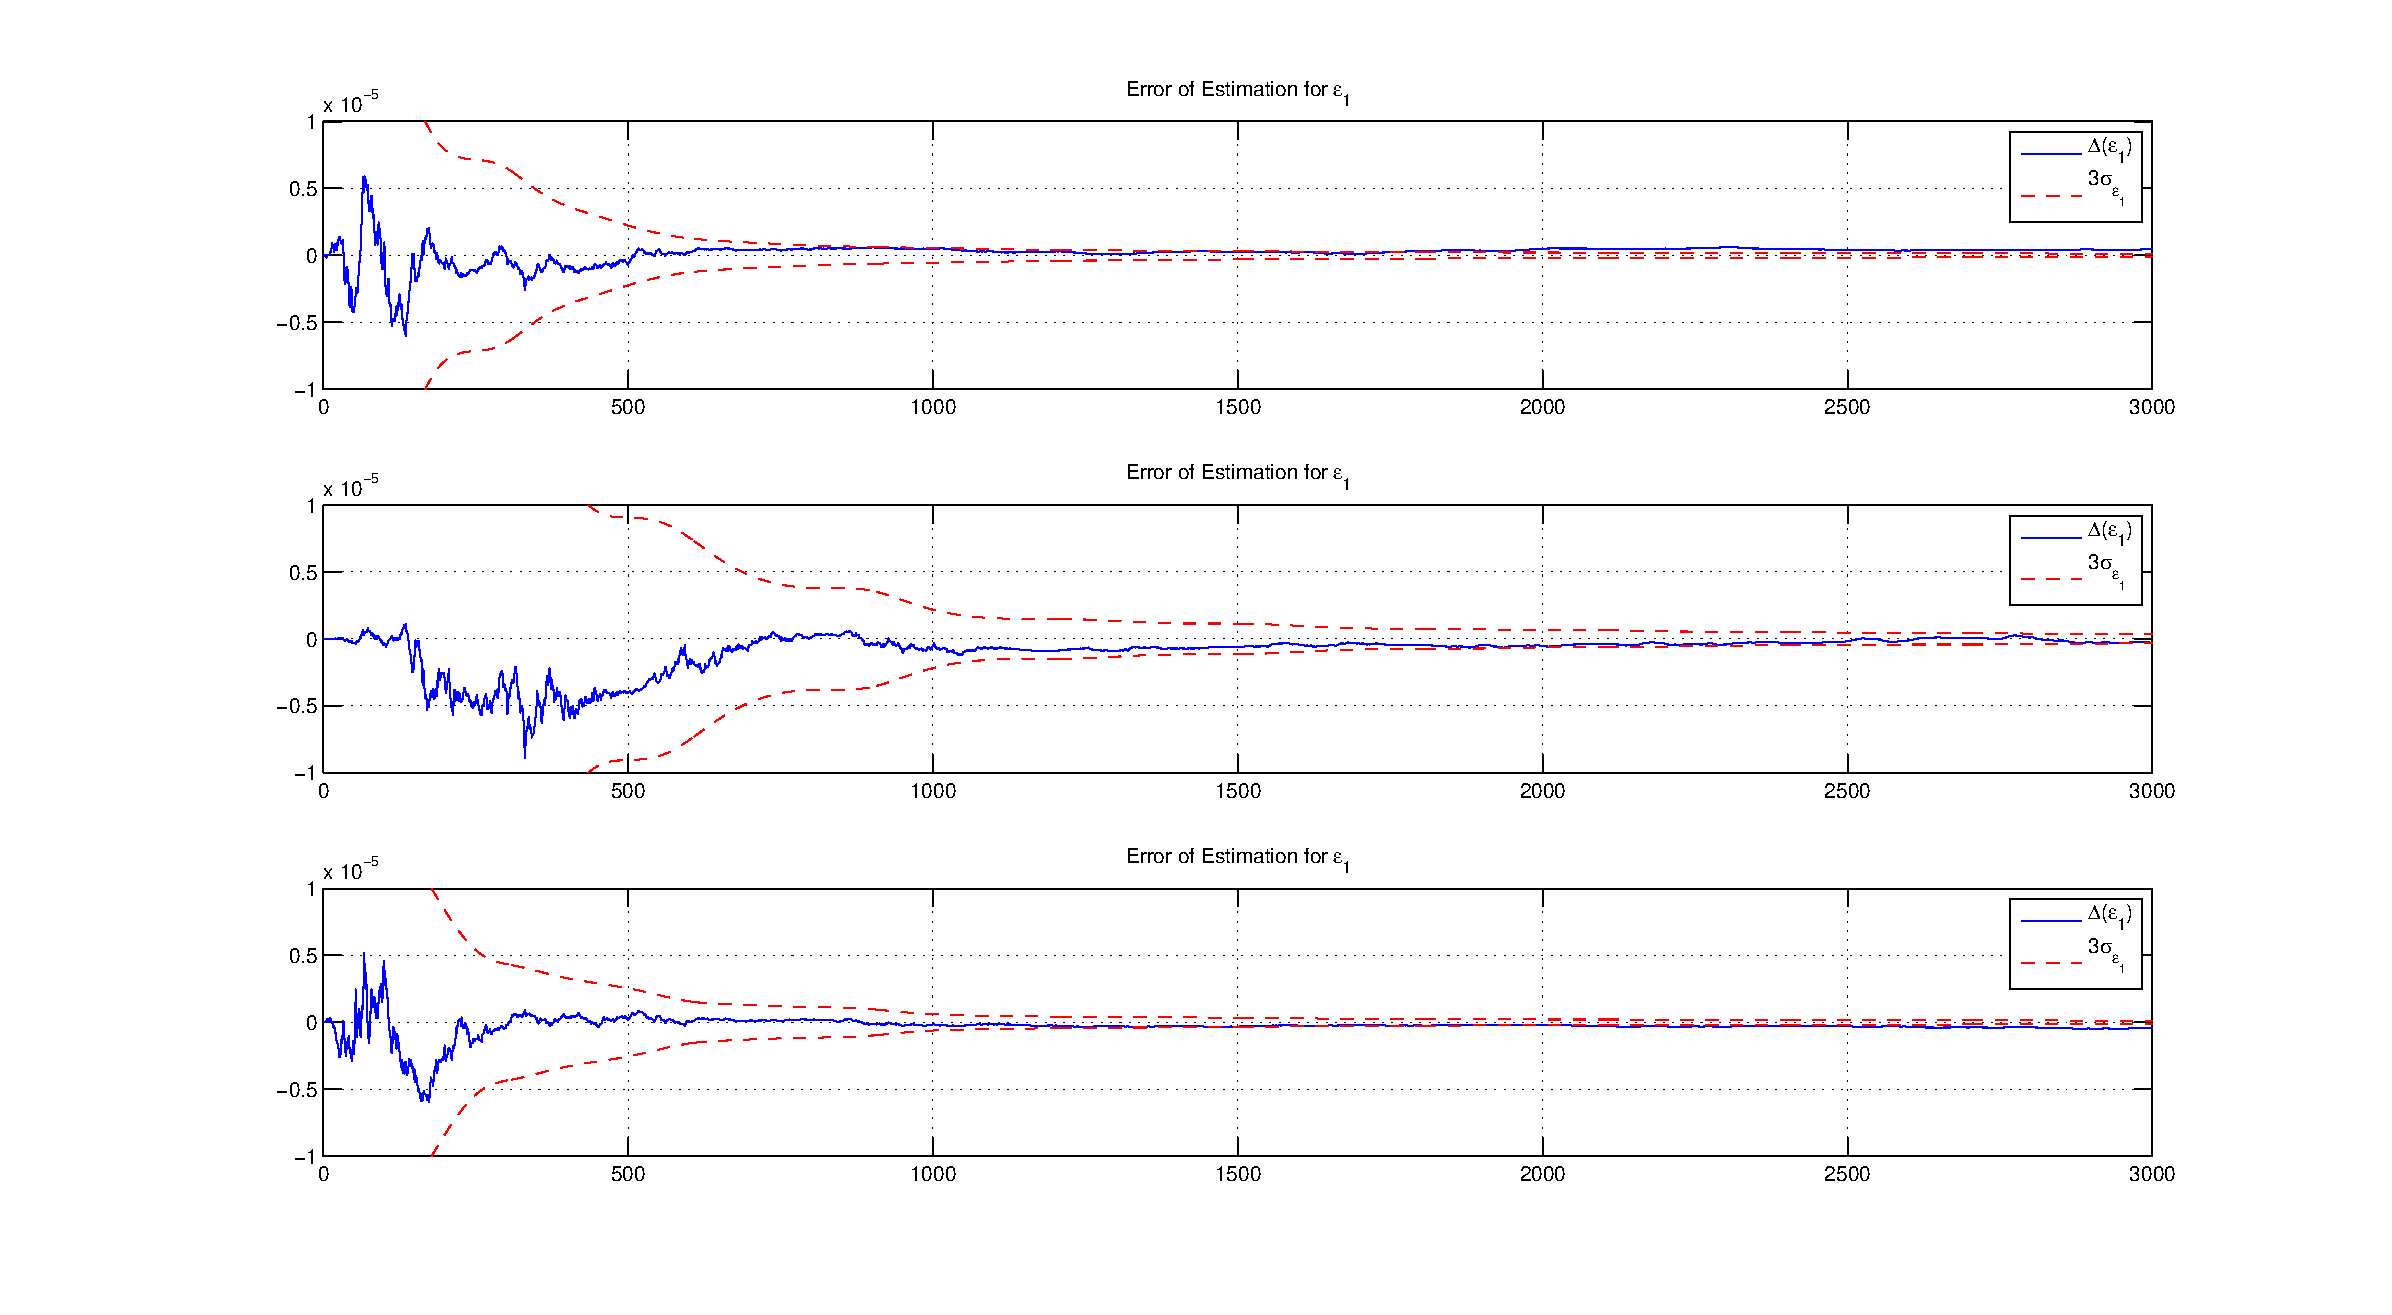
\includegraphics[scale=0.45]{ErrEstCovGyro}
\caption{Еволюції похибки оцінки дрейфів гіроскопів}
\label{fig:ErrEstCovGyro}
\end{figure}

\begin{figure}[H]
\centering
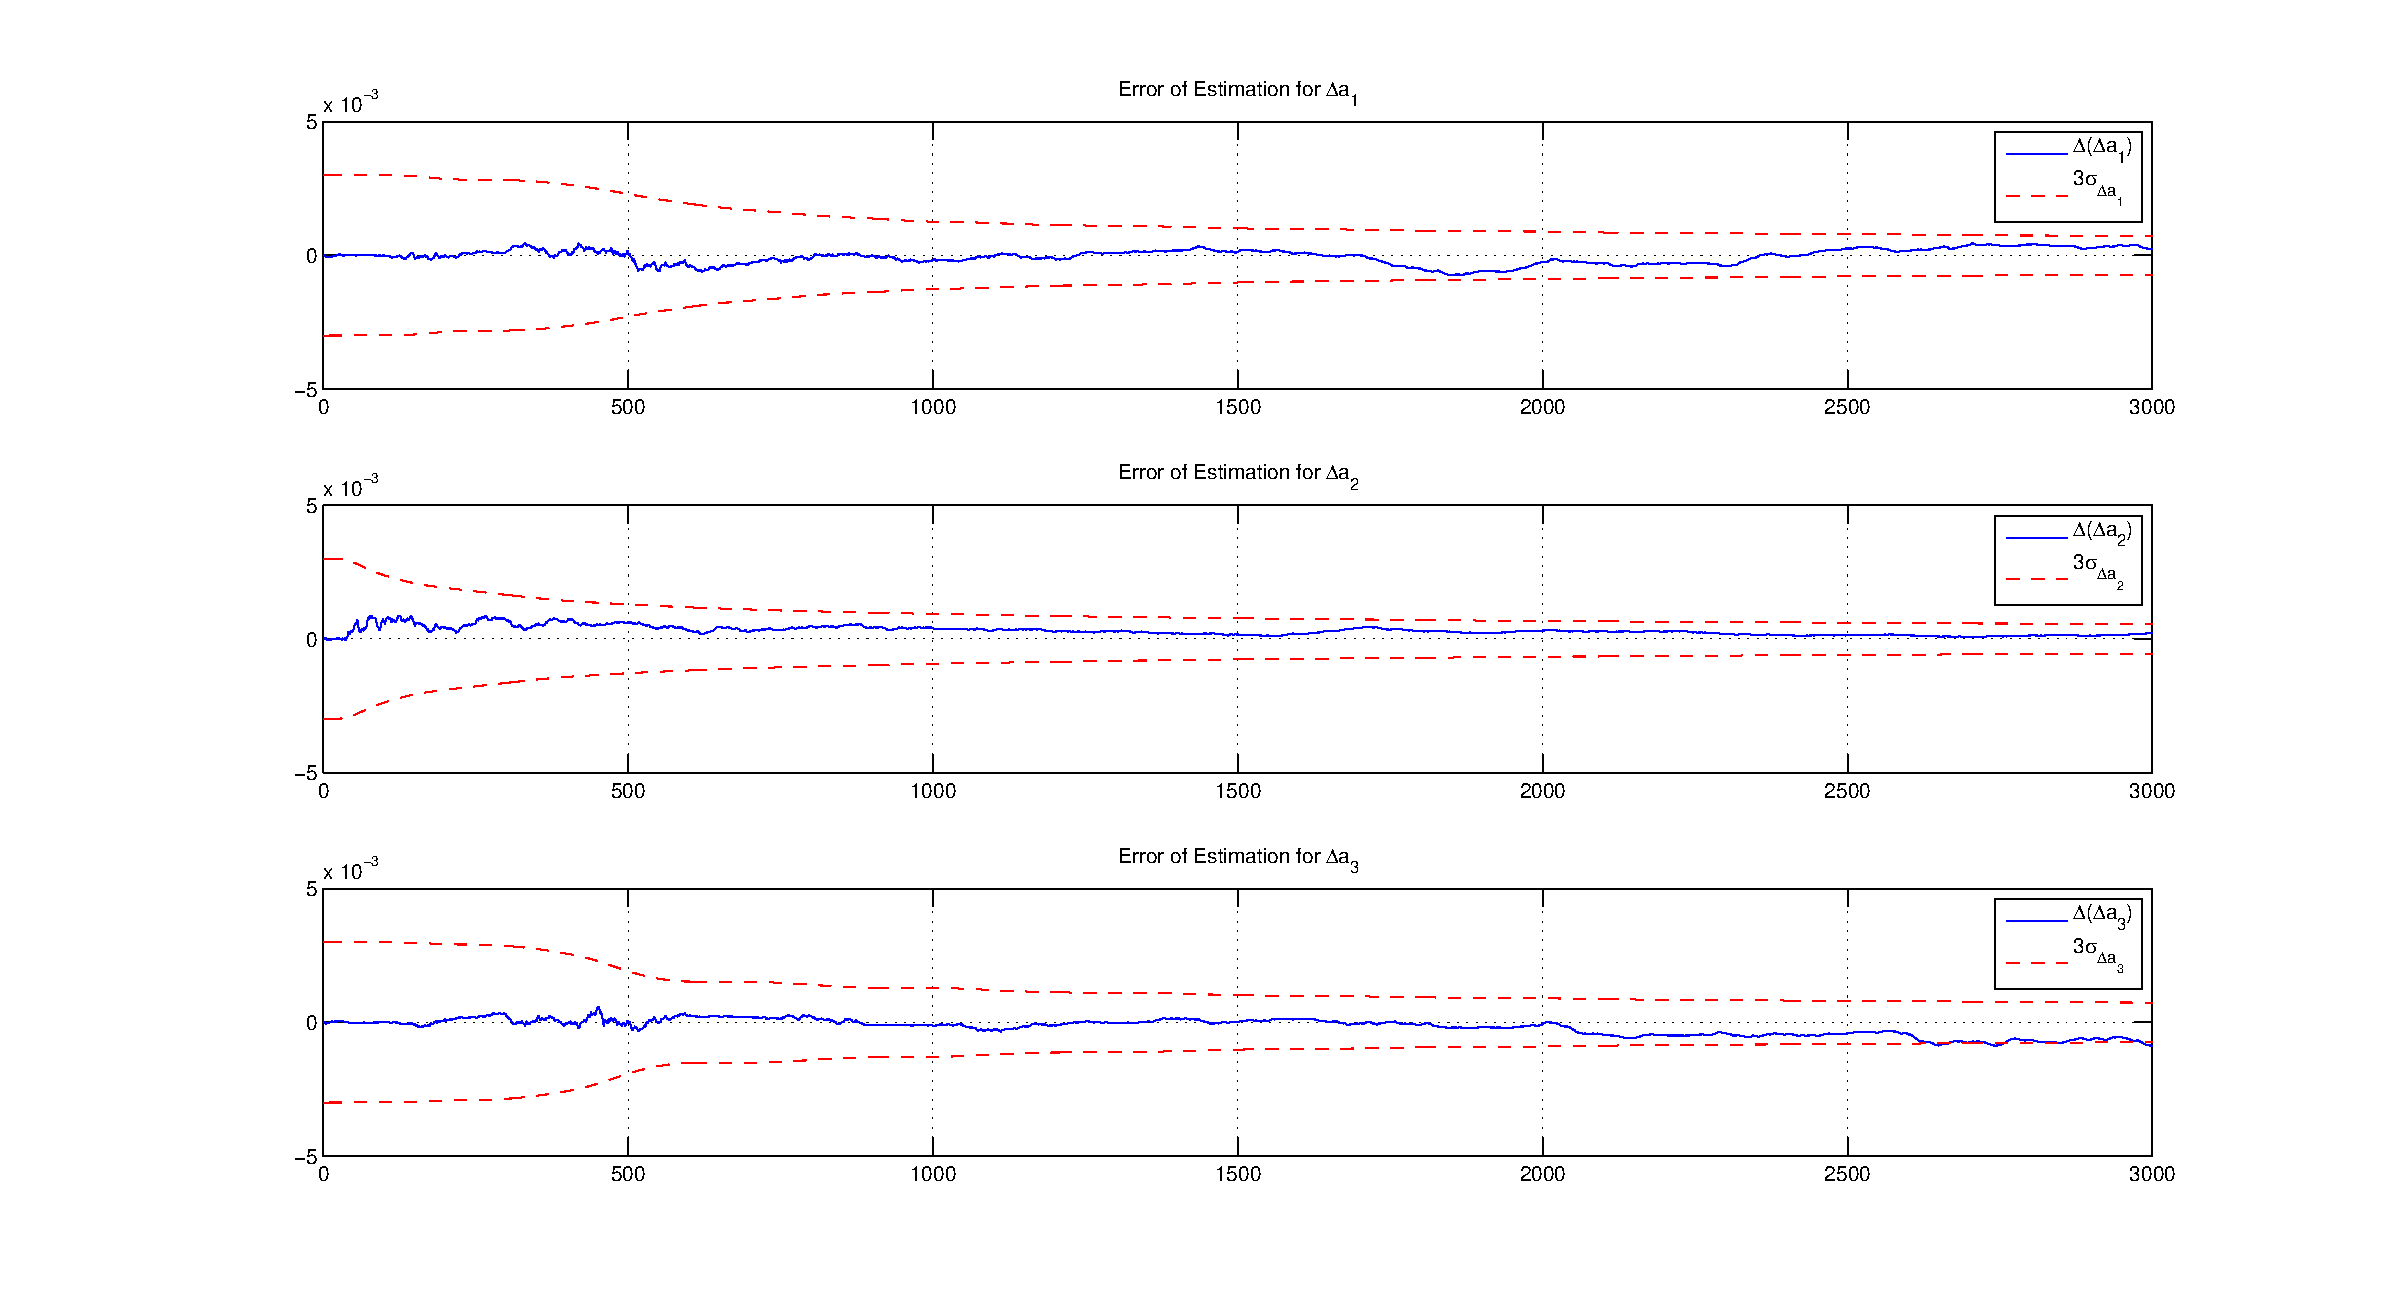
\includegraphics[scale=0.45]{ErrEstCovAcc}
\caption{Еволюції похибки оцінки дрейфів акселерометрів}
\label{fig:ErrEstCovAcc}
\end{figure}

Похибки оцінювання навігаційних параметрів, що спостерігаються, -- координат та складових швидкості сходяться до рівня корельованих складових похибок СНС, при цьому наявність корекції від барометричного висотоміра забезпечує стійкість вертикального каналу інтегрованої системи навігації. Одночасно оцінюються параметри, що не спостерігаються -- параметри кутової орієнтації, а також квазістаціонарні складові похибок ДПІ, які можна використовувати для польотного калібрування ДКШ та акселерометрів.  

Помилки оцінки крену, курсу і тангажа показані на рисунку \ref{fig:ErrEstAngle}

\begin{figure}[H]
\centering
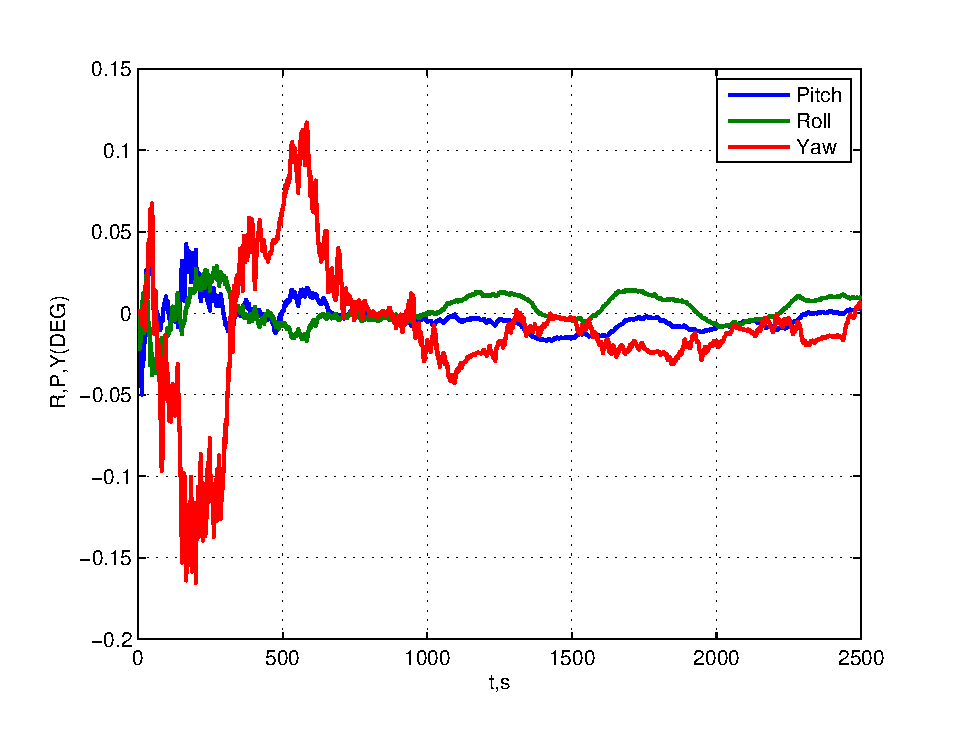
\includegraphics[scale=0.8]{ErrEstAngle}
\caption{Похибки оцінки кутів курсу, крену тангажу}
\label{fig:ErrEstAngle}
\end{figure}

При вимкненій супутниковій системі, але з фільтром Калмана та барометричним висотоміром, показання БІНС будуть наступними рис.\ref{fig:ins_kalman_ins}. Екстраполяція помилок за допомогою фільтра Калмана, значно покращує, результати навігаційної системи. В той час як автономно ІНС уходить, досить швидко, фільтр підтримує на прийнятному рівні +/-10 м на протязі 100 с. :

\begin{figure}[H]
\centering
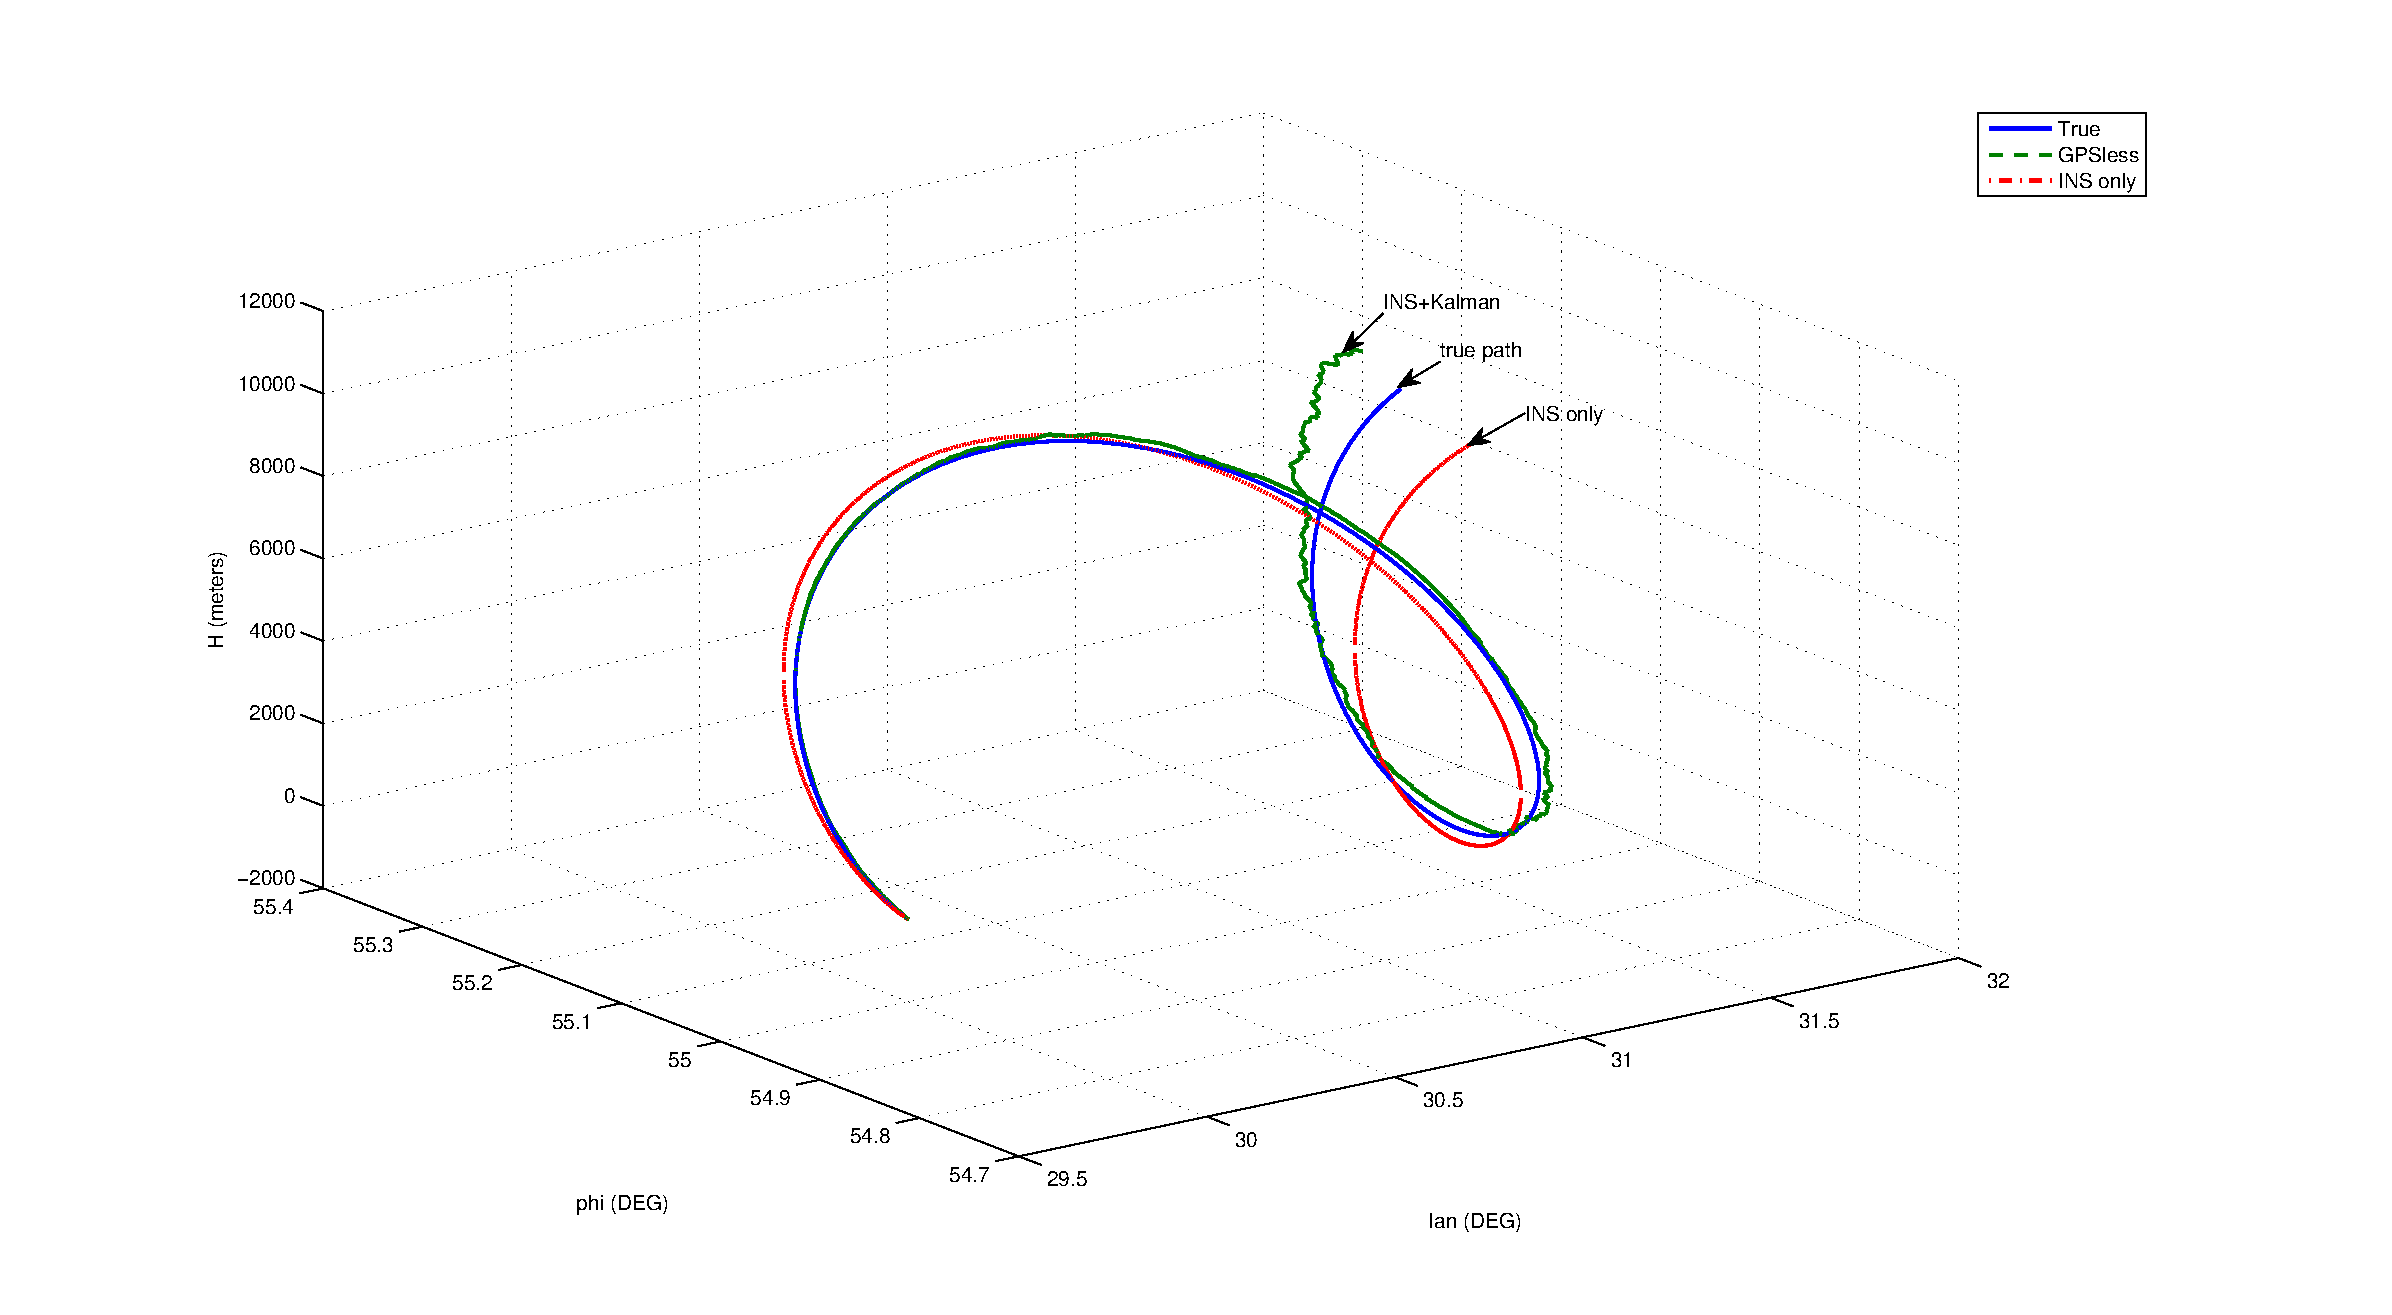
\includegraphics[scale=0.43]{ins_kalman_ins}
\caption{Траєкторія руху ЛА з вимкненою СНС}
\label{fig:ins_kalman_ins}
\end{figure}

Результати моделювання занесені до таблиці \ref{tab:results}, де вказані середньоквадратичні помилки по: координатам, швидкостям, орієнтації, дрейфів гіроскопів та акселерометрів після роботи системи на протязі 800с.

\begin{table}[H]
\centering
\caption{Середньоквадратичні помилки: }
\begin{tabular}{|p{50mm}|p{30mm}|p{30mm}|p{30mm}|} \hline
N&East&North&Height \\ \hline
Координати, м & 5.8792050244& 4.6476224404& 4.8677711489 \\ \hline 
Швидкості, м/с& 0.0236254078& 0.0235478062& 0.0231813797 \\ \hline 
Орієнтація, рад& 8.42E-005& 0.000133569& 0.0004735418 \\ \hline 
Дрейф ДКШ, рад/с& 2.50E-007& 1.28E-006 & 3.80E-007 \\ \hline 
Акселером, g & 0.00005007264& 0.0000344999 & 0.00004686141 \\ \hline 
\end{tabular}
\label{tab:results}
\end{table}

Аналіз результатів моделювання доказує працездатність розроблених алгоритмів комплексування. Дані таблиці \ref{tab:results} відповідають критеріям заданим в технічному завданні. Помилка по координаті не перевищує 5 метрів (1 сигма), по швидкості не більше 0.03 м/с, що відповідає рівню точності СНС.